%%%%%%%%%%%%%%%%%%%%%%%%%%%%%%%%%%%%%%%%%
% Beamer Presentation
% LaTeX Template
% Version 1.0 (10/11/12)
%
% This template has been downloaded from:
% http://www.LaTeXTemplates.com
%
% License:
% CC BY-NC-SA 3.0 (http://creativecommons.org/licenses/by-nc-sa/3.0/)
%
%%%%%%%%%%%%%%%%%%%%%%%%%%%%%%%%%%%%%%%%%

%----------------------------------------------------------------------------------------
%	PACKAGES AND THEMES
%----------------------------------------------------------------------------------------

\documentclass{beamer}

\mode<presentation> {

% The Beamer class comes with a number of default slide themes
% which change the colors and layouts of slides. Below this is a list
% of all the themes, uncomment each in turn to see what they look like.

%\usetheme{default}
%\usetheme{AnnArbor}
%\usetheme{Antibes}
%\usetheme{Bergen}
%\usetheme{Berkeley}
%\usetheme{Berlin}
%\usetheme{Boadilla}
%\usetheme{CambridgeUS}
%\usetheme{Copenhagen}
%\usetheme{Darmstadt}
%\usetheme{Dresden}
%\usetheme{Frankfurt}
%\usetheme{Goettingen}
%\usetheme{Hannover}
%\usetheme{Ilmenau}
%\usetheme{JuanLesPins}
%\usetheme{Luebeck}
\usetheme{Madrid}
%\usetheme{Malmoe}
%\usetheme{Marburg}
%\usetheme{Montpellier}
%\usetheme{PaloAlto}
%\usetheme{Pittsburgh}
%\usetheme{Rochester}
%\usetheme{Singapore}
%\usetheme{Szeged}
%\usetheme{Warsaw}

% As well as themes, the Beamer class has a number of color themes
% for any slide theme. Uncomment each of these in turn to see how it
% changes the colors of your current slide theme.

%\usecolortheme{albatross}
%\usecolortheme{beaver}
%\usecolortheme{beetle}
%\usecolortheme{crane}
%\usecolortheme{dolphin}
%\usecolortheme{dove}
%\usecolortheme{fly}
%\usecolortheme{lily}
%\usecolortheme{orchid}
%\usecolortheme{rose}
%\usecolortheme{seagull}
%\usecolortheme{seahorse}
%\usecolortheme{whale}
%\usecolortheme{wolverine}

%\setbeamertemplate{footline} % To remove the footer line in all slides uncomment this line
%\setbeamertemplate{footline}[page number] % To replace the footer line in all slides with a simple slide count uncomment this line

%\setbeamertemplate{navigation symbols}{} % To remove the navigation symbols from the bottom of all slides uncomment this line
}

\usepackage{graphicx} % Allows including images
\usepackage{booktabs} % Allows the use of \toprule, \midrule and \bottomrule in tables

%----------------------------------------------------------------------------------------
%	TITLE PAGE
%----------------------------------------------------------------------------------------

\title[MongoDB vs OrientDB]{MongoDB vs OrientDB} % The short title appears at the bottom of every slide, the full title is only on the title page

\author{Stefano Campese} % Your name
%\institute[] % Your institution as it will appear on the bottom of every slide, may be shorthand to save space
%{
%University of California \\ % Your institution for the title page
%\medskip
%\textit{john@smith.com} % Your email address
%}
\date{\today} % Date, can be changed to a custom date

\begin{document}

\begin{frame}
\titlepage % Print the title page as the first slide
\end{frame}

\begin{frame}
\frametitle{Overview} % Table of contents slide, comment this block out to remove it
\tableofcontents % Throughout your presentation, if you choose to use \section{} and \subsection{} commands, these will automatically be printed on this slide as an overview of your presentation
\end{frame}

%----------------------------------------------------------------------------------------
%	PRESENTATION SLIDES
%----------------------------------------------------------------------------------------

%------------------------------------------------
\section{Introduzione} % Sections can be created in order to organize your presentation into discrete blocks, all sections and subsections are automatically printed in the table of contents as an overview of the talk
%------------------------------------------------

%\subsection{Subsection Example} % A subsection can be created just before a set of slides with a common theme to further break down your presentation into chunks

\begin{frame}
\frametitle{MongoDB}
Nato nel 2009, è uno dei database documentali più conosciuto e utilizzato nel mondo le sue caratteristiche principali sono.
\begin{itemize}
\item Linguaggio di implementazione C++
\item Modello di database \emph{Document Store}
\item Database NO-SQL e Non relazionale
\item Assenza di Transazioni ACID
\item Linguaggio Query ad hoc
\item Aggregazione
\item Indici unici
\end{itemize}
\end{frame}

%------------------------------------------------

\begin{frame}
\frametitle{OrientDB}
Nato nel 2010, è un ibrido tra un database documentale un database a grafi.\\
Le sue caratteristiche principali sono.
\begin{itemize}
\item Linguaggio di implementazione Java
\item Modello di database \emph{Document Store - Graph DBMS}
\item Database NO-SQL 
\item Linguaggio Query simile a SQL
\item Presenza di Transazioni ACID
\item Indicizzazione che permette il multithread
\item Trigger
\end{itemize}
\end{frame}

%------------------------------------------------
\section{Sciegliere il DB corretto}

\begin{frame}
\frametitle{Quando usare MongoDB}
\begin{columns}[c] % The "c" option specifies centered vertical alignment while the "t" option is used for top vertical alignment

\column{.45\textwidth} % Left column and width
\textbf{Perchè usare MongoDB?}
\begin{enumerate}
\item Grande quantità di dati
\item Non servono Transazioni
\item Non servono relazioni
\item Modello di Sviluppo Agile
\item Scalabilità
\item Prestazioni
\end{enumerate}

\column{.5\textwidth} % Right column and width

\includegraphics[width=1.2\linewidth]{mongodb.png}

\end{columns}
\end{frame}


%------------------------------------------------

\begin{frame}
\frametitle{Quando usare OrientDB}
\begin{columns}[c] % The "c" option specifies centered vertical alignment while the "t" option is used for top vertical alignment

\column{.45\textwidth} % Left column and width
\textbf{Perchè usare OrientDB?}
\begin{enumerate}
\item Grande quantità di dati
\item servono Transazioni
\item servono relazioni
\item Modello di Sviluppo Agile
\item Scalabilità
\item Prestazioni (JOIN incluse)
\item Linguaggio Query
\item Classi di Oggetti
\end{enumerate}

\column{.5\textwidth} % Right column and width

\includegraphics[width=1\linewidth]{orientdb.png}

\end{columns}
\end{frame}

%------------------------------------------------
\section{MongoDB VS OrientDB}
%------------------------------------------------

\begin{frame}
\frametitle{MongoDB VS OrientDB}

\begin{block}{Relazioni}
\begin{itemize}
\item OrientDB: Relazioni con \emph{puntatori} tra JSON
\item MongoDB: \emph{Indici} scritti su file
\end{itemize}
\end{block}

\begin{block}{Linguaggio}
\begin{itemize}
\item OrientDB: linguaggio simil SQL
\item MongoDB: liguaggio propietario 
\end{itemize}
\end{block}

\begin{block}{Gestione Memoria}
\begin{itemize}
\item OrientDB: usa tecnica chiamata PLOCAL
\item MongoDB:  usa tecnica chiamata LOCAL
\end{itemize}
\end{block}

\begin{block}{Inidicizzazione}
\begin{itemize}
\item OrientDB: tre algoritmi (SB-tree, Hash index ,Lucene)
\item MongoDB:  un algoritmo (B-tree)
\end{itemize}
\end{block}

\end{frame}


%------------------------------------------------
\section{Esempi}
%------------------------------------------------

\begin{frame}
\frametitle{Figure}
\begin{figure}
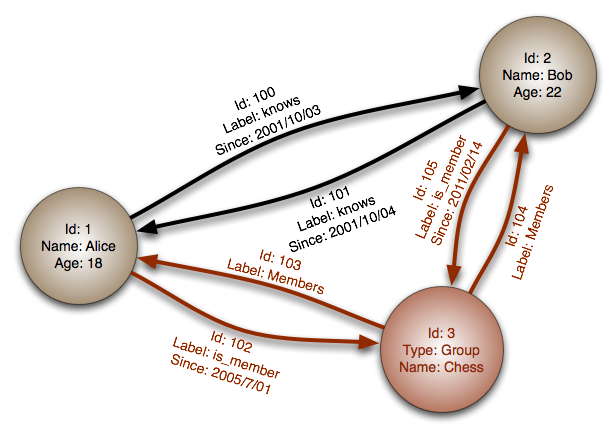
\includegraphics[width=0.8\linewidth]{GraphDatabase_PropertyGraph.png}
\caption{Esmepio di vertici OrientDB}
\end{figure}
\end{frame}

%------------------------------------------------

\begin{frame}
\frametitle{Figure}
\begin{figure}
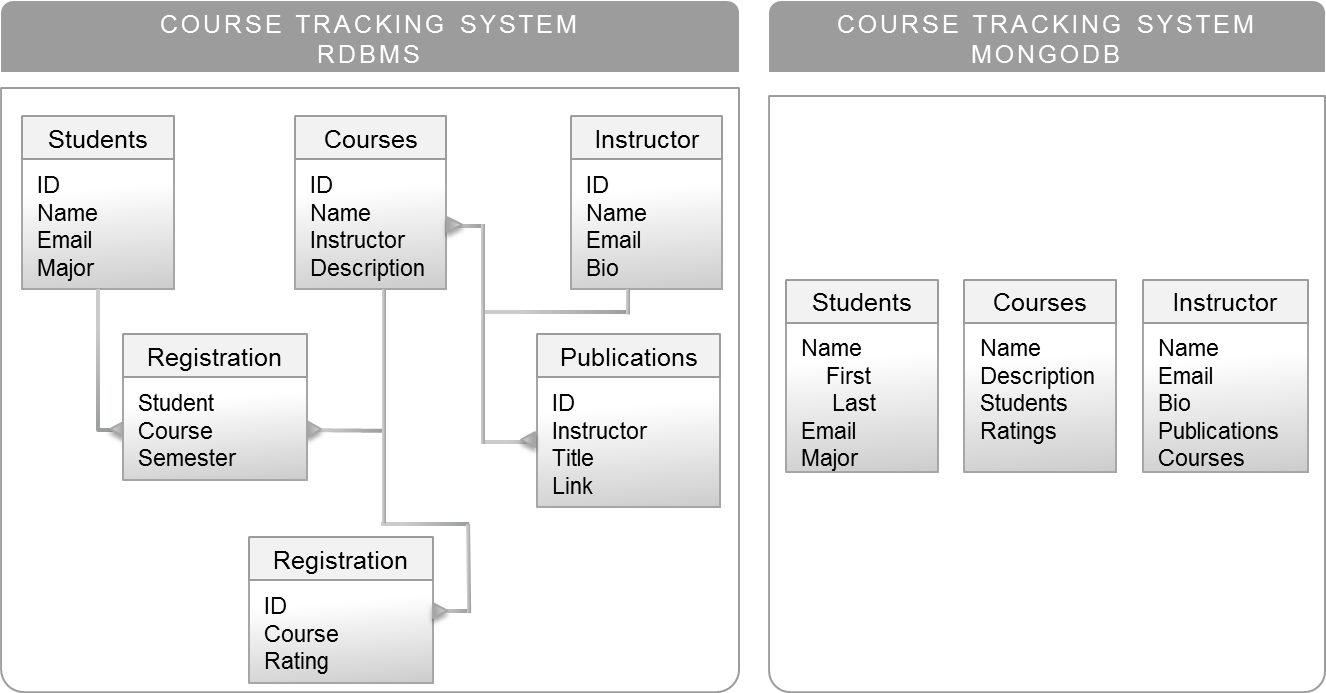
\includegraphics[width=0.8\linewidth]{01_mongodb_courses.png}
\caption{Esmepio conversione SQL a MongoDB}
\end{figure}
\end{frame}


%------------------------------------------------

%\begin{frame}
%\frametitle{References}
%\footnotesize{
%\begin{thebibliography}{99} % Beamer does not support BibTeX so references must be inserted manually as below
%\bibitem[Smith, 2012]{p1} John Smith (2012)
%\newblock Title of the publication
%\newblock \emph{Journal Name} 12(3), 45 -- 678.
%\end{thebibliography}
%}
%\end{frame}

%------------------------------------------------

\begin{frame}
\Huge{\centerline{Fine}}
\end{frame}

%----------------------------------------------------------------------------------------

\end{document}